\documentclass[11pt,paper=a4,answers]{exam}
\usepackage{graphicx,lastpage}
\usepackage{upgreek}
\usepackage{censor}
\usepackage{gensymb}
\usepackage{amsmath}
\usepackage{multicol}
\usepackage{enumitem}
 \usepackage{pgfplots}
\pgfplotsset{compat=1.18}
\usepackage{tasks}
\usepackage{adjustbox}
\usepackage{xcolor}
\usepackage{tfrupee}
\setlength{\voffset}{0.25in}
\usepackage{tabularx}
\newcolumntype{Y}{>{\centering\arraybackslash}X}
%==============================================================
% Customise Non-Essential Packages Below
% =============================================================
\usepackage[most]{tcolorbox}
\usepackage{eso-pic}
\usepackage{tikz}
\AddToShipoutPictureBG{%
\begin{tikzpicture}[remember picture,overlay]
\foreach \x in {-8,-4,0,4,8,12,16,20}
\foreach \y in {-8,-4,0,4,8,12,16,20} {
\node[opacity=0.05,rotate=45,anchor=center] at ([xshift=\x cm,yshift=\y cm]current page.center) {%
\begin{minipage}{2cm}
\centering
\includegraphics[width=2cm]{images/logo_black.png}\\
\small preppeo.com
\end{minipage}%
};
}
\end{tikzpicture}%
}
\printanswers

%==============================================================
% Customise Non-Essential Packages Above
% =============================================================
\definecolor{svgray}{rgb}{0.90, 0.90, 0.90}
\graphicspath{{images/}}

\usepackage[normalem]{ulem}
\renewcommand\ULthickness{1pt}   %%---> For changing thickness of underline
\setlength\ULdepth{3.5ex}%\maxdimen ---> For changing depth of underline
\renewcommand{\baselinestretch}{1}
\chead{
\includegraphics[scale=0.1,height=2cm ]{logo.png}
}
\pagestyle{empty}

\pagestyle{headandfoot}
\headrule
\cfoot{W: https://preppeo.com; M: +91-8130711689}

\begin{document}
%==============================================================
% Customise Question paper details below this
% =============================================================
\begin{center}
    \centering
    \renewcommand{\arraystretch}{1.5}
    \begin{tabularx}{\textwidth}{YYY}
    & \normalsize\bf{{\Large{{Quantitative Reasoning}}}} & \\
    By Preppeo & \normalsize\bf{MOCK } & GRE\\
    \normalsize{\textbf{Questions:} 15 ( Section 2 : 15} & \normalsize{\textbf{Marks:} 15 } & \normalsize{\textbf{Time:}  minutes } \\
    \end{tabularx}
\end{center}
\par\noindent\rule{\textwidth}{1pt}
% =============================================================
% Customise Question paper details above this
% =============================================================

\begin{questions}
\pointsinrightmargin
\pointsdroppedatright
\marksnotpoints
\pointpoints{mark}{marks}
\pointformat{\boldmath\themarginpoints}
\bracketedpoints

% =============================================================
% Question Begin
% =============================================================

\section*{Section 2 - Mock 9 Set 3 (Very Very Hard)}

% --- QUANTITY COMPARISON (5 QUESTIONS) ---

%Q: 1
\question
Eight women and two men are available to serve on a committee. If three people are picked at random to form the committee:
\vspace{5pt}\\
\textbf{Quantity A: } The probability that the committee includes at least one man \\
\vspace{5pt}
\textbf{Quantity B: } 0.5

\begin{tasks}(1)
\task[A)] Quantity A is greater
\task[B)] Quantity B is greater
\task[C)] The two quantities are equal
\task[D)] The relationship cannot be determined
\end{tasks}

\begin{solution}
To find the probability of "at least one man," it is easiest to subtract the probability of "no men" (all women) from 1.
\vspace{5pt}
\begin{center}
Total people = 8 women + 2 men = 10.
\vspace{5pt}
Total ways to choose 3 people from 10: 
\vspace{5pt}
$\binom{10}{3} = \dfrac{10 \times 9 \times 8}{3 \times 2 \times 1} = 120$.
\vspace{10pt}
Ways to choose 3 women from 8:
\vspace{5pt}
$\binom{8}{3} = \dfrac{8 \times 7 \times 6}{3 \times 2 \times 1} = 56$.
\vspace{10pt}
$P(\text{All Women}) = \dfrac{56}{120} = \dfrac{7}{15}$.
\vspace{10pt}
$P(\text{At least one man}) = 1 - \dfrac{7}{15} = \dfrac{8}{15}$.
\vspace{5pt}
Convert to decimal: $8 \div 15 \approx 0.533$.
\end{center}
\vspace{5pt}
Quantity A ($\approx 0.533$) is greater than Quantity B ($0.5$).

Answer: \colorbox{yellow!100}{A}
\end{solution}

\vspace{1cm}

%Q: 2
\question
\begin{center}
\begin{tikzpicture}[scale=0.8]
\begin{axis}[
    axis lines=middle,
    xlabel=$x$, ylabel=$y$,
    xmin=-5, xmax=5,
    ymin=-2, ymax=10,
    grid=major,
    width=8cm, height=6cm
]
\addplot[domain=-3:3, samples=100, ultra thick, red] {(x-1)^2 + 2};
\node[circle, fill, inner sep=1.5pt, label=below right:{$(1,2)$}] at (axis cs:1,2) {};
\node[circle, fill, inner sep=1.5pt, label=left:{$(0,3)$}] at (axis cs:0,3) {};
\end{axis}
\end{tikzpicture}
\end{center}
The parabola above is defined by $y = a(x-h)^2 + k$.
\vspace{5pt}\\
\textbf{Quantity A: } $a + h + k$ \\
\vspace{5pt}
\textbf{Quantity B: } 4

\begin{tasks}(1)
\task[A)] Quantity A is greater
\task[B)] Quantity B is greater
\task[C)] The two quantities are equal
\task[D)] The relationship cannot be determined
\end{tasks}

\begin{solution}
Identify the vertex $(h, k)$ from the graph: the peak is at $(1, 2)$, so $h = 1$ and $k = 2$.
\vspace{5pt}
\begin{center}
Equation: $y = a(x - 1)^2 + 2$.
\vspace{5pt}
Use the y-intercept $(0, 3)$ to find $a$:
\vspace{5pt}
$3 = a(0 - 1)^2 + 2 \implies 3 = a(1) + 2 \implies a = 1$.
\vspace{10pt}
Quantity A: $a + h + k = 1 + 1 + 2 = 4$.
\end{center}
\vspace{5pt}
Quantity A is 4 and Quantity B is 4. They are equal.

Answer: \colorbox{yellow!100}{C}
\end{solution}

\vspace{1cm}

%Q: 3
\question
$x$ is a non-zero integer and $0 < y < 1$.
\vspace{5pt}\\
\textbf{Quantity A: } $x^2 / y$ \\
\vspace{5pt}
\textbf{Quantity B: } 1

\begin{tasks}(1)
\task[A)] Quantity A is greater
\task[B)] Quantity B is greater
\task[C)] The two quantities are equal
\task[D)] The relationship cannot be determined
\end{tasks}

\begin{solution}
Since $x$ is a non-zero integer, $x^2$ must be at least 1 ($1, 4, 9, \dots$).
\vspace{5pt}
\begin{center}
Since $y$ is a fraction between 0 and 1, dividing any number by $y$ increases its value.
\vspace{5pt}
The minimum possible value for Quantity A occurs when $x^2$ is smallest (1) and $y$ is largest (approaching 1).
\vspace{5pt}
Even if $y = 0.99$, $1 / 0.99 > 1$.
\end{center}
\vspace{5pt}
Therefore, $x^2 / y$ will always be strictly greater than 1.

Answer: \colorbox{yellow!100}{A}
\end{solution}

\vspace{1cm}

%Q: 4
\question
An inventory contains 100 different coins.
\vspace{5pt}\\
\textbf{Quantity A: } The number of possible collections of 56 coins that can be selected \\
\vspace{5pt}
\textbf{Quantity B: } The number of possible collections of 44 coins that can be selected

\begin{tasks}(1)
\task[A)] Quantity A is greater
\task[B)] Quantity B is greater
\task[C)] The two quantities are equal
\task[D)] The relationship cannot be determined
\end{tasks}

\begin{solution}
This question tests the combinatorial identity $\binom{n}{k} = \binom{n}{n-k}$.
\vspace{5pt}
\begin{center}
Quantity A = $\binom{100}{56}$
\vspace{5pt}
Quantity B = $\binom{100}{44}$
\vspace{10pt}
Since $100 - 56 = 44$, the number of ways to choose 56 coins to \textit{keep} is mathematically identical to the number of ways to choose 44 coins to \textit{leave behind}.
\end{center}
\vspace{5pt}
The two quantities are equal.

Answer: \colorbox{yellow!100}{C}
\end{solution}

\vspace{1cm}

%Q: 5
\question
$x + y = 10$ and $|x + y| = 10$. $x \geq 0$ and $z < y - x$.
\vspace{5pt}\\
\textbf{Quantity A: } $z$ \\
\vspace{5pt}
\textbf{Quantity B: } 10

\begin{tasks}(1)
\task[A)] Quantity A is greater
\task[B)] Quantity B is greater
\task[C)] The two quantities are equal
\task[D)] The relationship cannot be determined
\end{tasks}

\begin{solution}
From $x+y=10$ and $x \geq 0$, we know the maximum possible value for $y-x$ occurs when $x$ is smallest.
\vspace{5pt}
\begin{center}
If $x = 0$, then $y = 10$, and $y - x = 10$.
\vspace{5pt}
The condition $z < y - x$ becomes $z < 10$.
\vspace{5pt}
If $x > 0$ (e.g., $x=2$), then $y=8$, and $y - x = 6$. The condition becomes $z < 6$.
\end{center}
\vspace{5pt}
In all valid scenarios for $x$ and $y$, $z$ must be strictly less than a value that is at most 10.
\vspace{5pt}
Therefore, $z$ is always less than 10.

Answer: \colorbox{yellow!100}{B}
\end{solution}

\vspace{1cm}

% --- MCQ SINGLE CHOICE (5 QUESTIONS) ---

%Q: 6
\question
A solid right circular cylinder with height 9 and radius 2 is cut into three new cylinders of equal and uniform height. How much new surface area is created?

\begin{tasks}(1)
\task[A)] $4\pi$ \task[B)] $8\pi$ \task[C)] $12\pi$ \task[D)] $16\pi$ \task[E)] $24\pi$
\end{tasks}

\begin{solution}
\begin{center}
Each time a cylinder is cut horizontally, two new circular faces are created.
\vspace{5pt}
To create three new cylinders, the original must be cut twice.
\vspace{5pt}
Total new faces = $2 \text{ cuts} \times 2 \text{ faces per cut} = 4 \text{ faces}$.
\vspace{5pt}
Area of one circular face = $\pi r^2 = \pi (2^2) = 4\pi$.
\vspace{5pt}
New surface area = $4 \times 4\pi = 16\pi$.
\end{center}

Answer: \colorbox{yellow!100}{D}
\end{solution}

\vspace{1cm}

%Q: 7
\question
A robot's rate of polishing is $3/5$ that of another robot. Working together, they polish 88 pounds of gemstones in 6 minutes. How many minutes would it take the slower robot alone to polish 165 pounds?

\begin{tasks}(1)
\task[A)] 15.75 \task[B)] 18 \task[C)] 25 \task[D)] 30 \task[E)] 40
\end{tasks}

\begin{solution}
\begin{center}
Let $R_B$ be the rate of the faster robot and $R_A = 0.6R_B$ be the slower.
\vspace{5pt}
Combined rate: $R_A + R_B = 1.6R_B = 88/6 = 44/3 \text{ lbs/min}$.
\vspace{5pt}
$R_B = (44/3) / 1.6 = (44/3) / (8/5) = 220 / 24 = 55/6 \text{ lbs/min}$.
\vspace{5pt}
$R_A = 0.6 \times (55/6) = (3/5) \times (55/6) = 11/2 = 5.5 \text{ lbs/min}$.
\vspace{10pt}
Time for A to polish 165 lbs: $165 / 5.5 = 30 \text{ minutes}$.
\end{center}

Answer: \colorbox{yellow!100}{D}
\end{solution}

\vspace{1cm}

%Q: 8
\question
In a certain group, the ratio of women to men is 5 to 6, and the ratio of left-handed to right-handed people is 7 to 9. If everyone is either left- or right-handed, what is the minimum number of people in the group?

\begin{tasks}(1)
\task[A)] 11 \task[B)] 16 \task[C)] 66 \task[D)] 176 \task[E)] 196
\end{tasks}

\begin{solution}
The total number of people must be a multiple of the sum of the ratio parts for both categories.
\vspace{5pt}
\begin{center}
Women/Men: $5 + 6 = 11$.
\vspace{5pt}
Left/Right: $7 + 9 = 16$.
\vspace{5pt}
Minimum total = Least Common Multiple of 11 and 16.
\vspace{5pt}
$\text{LCM}(11, 16) = 11 \times 16 = 176$.
\end{center}

Answer: \colorbox{yellow!100}{D}
\end{solution}

\vspace{1cm}

%Q: 9
\question
Julian cuts a 10-inch square piece of paper in half along the diagonal, then cuts one of those halves in half again from the corner to the midpoint of the opposite side. What is the perimeter of one of the smallest triangles?

\begin{tasks}(1)
\task[A)] 10 \task[B)] $10\sqrt{2}$ \task[C)] 20 \task[D)] $10 + 10\sqrt{2}$ \task[E)] $10 + 5\sqrt{2}$
\end{tasks}

\begin{solution}

\begin{center}
First cut: Creates two isosceles right triangles with legs 10 and hypotenuse $10\sqrt{2}$.
\vspace{5pt}
Second cut: Bisects the hypotenuse ($10\sqrt{2}$) into two segments of $5\sqrt{2}$.
\vspace{5pt}
The altitude to the hypotenuse of an isosceles right triangle is also $5\sqrt{2}$.
\vspace{5pt}
Smallest triangle sides: $10, 5\sqrt{2}, 5\sqrt{2}$.
\vspace{5pt}
$\text{Perimeter} = 10 + 5\sqrt{2} + 5\sqrt{2} = 10 + 10\sqrt{2}$.
\end{center}

Answer: \colorbox{yellow!100}{D}
\end{solution}

\vspace{1cm}

%Q: 10
\question
A polygon has 12 edges. How many different diagonals can be drawn from its vertices?

\begin{tasks}(1)
\task[A)] 54 \task[B)] 66 \task[C)] 108 \task[D)] 132 \task[E)] 144
\end{tasks}

\begin{solution}
Use the diagonal formula for an $n$-sided polygon: $d = \dfrac{n(n - 3)}{2}$.
\vspace{5pt}
\begin{center}
$n = 12$.
\vspace{5pt}
$d = \dfrac{12(12 - 3)}{2} = \dfrac{12 \times 9}{2} = 6 \times 9 = 54$.
\end{center}

Answer: \colorbox{yellow!100}{A}
\end{solution}

\vspace{1cm}

% --- MCQ MULTIPLE CHOICE (1 QUESTION) ---

%Q: 11
\question
The average age of buildings on a block is greater than 40 years. Four buildings are 2 years old and none are older than 80. Which of the following could be the number of buildings on the block?
Indicate \textbf{all} such values.

\begin{tasks}(1)
\task[A)] 6
\task[B)] 8
\task[C)] 11
\task[D)] 40
\end{tasks}

\begin{solution}
Let $n$ be the number of buildings and $S$ be the sum of their ages. $S / n > 40 \implies S > 40n$.
\vspace{5pt}
\begin{center}
$S = (4 \times 2) + \text{remaining buildings ages} \leq 8 + (n - 4) \times 80$.
\vspace{5pt}
$40n < 8 + 80n - 320 \implies 40n > 312 \implies n > 7.8$.
\end{center}
Possible values for $n$ are 8, 11, and 40.

Answer: \colorbox{yellow!100}{B, C, D}
\end{solution}

\vspace{1cm}

% --- INPUT QUESTION (1 QUESTION) ---

%Q: 12
\question
If the equation of a parabola is $y = (x - h)^2 + k$ and $(-3, n)$ is a point on the parabola with vertex $(2, 16)$, what is the value of $n$?

\begin{solution}
\begin{center}
Vertex $(h, k) = (2, 16)$.
\vspace{5pt}
Equation: $y = (x - 2)^2 + 16$.
\vspace{5pt}
Substitute point $(-3, n)$:
\vspace{5pt}
$n = (-3 - 2)^2 + 16 = (-5)^2 + 16 = 25 + 16 = 41$.
\end{center}

Answer: \colorbox{yellow!100}{41}
\end{solution}

\vspace{1cm}

% --- DATA INTERPRETATION (3 QUESTIONS) ---
\textbf{Questions 13-15 refer to the following scatter plot.}

\begin{center}
\begin{tikzpicture}
\begin{axis}[
    title={Manufacturing Defects vs. Experience},
    xlabel={Experience (Hours)},
    ylabel={Defects per 1,000},
    grid=major,
    xmin=0, xmax=16000,
    ymin=0, ymax=60,
    width=10cm, height=6cm
]
\addplot[only marks, mark=*, blue] coordinates {
    (1000,15) (2000,28) (4000,42) (6000,50) (8000,52) (10000,48) (12000,30) (14000,12)
};
\addplot[thick, red, domain=0:16000, samples=100] {-0.000001*(x-8000)^2 + 52.5};
\end{axis}
\end{tikzpicture}
\end{center}

%Q: 13
\question
Approximately how many defects per 1,000 are produced by an operator with 12,000 hours of experience?

\begin{tasks}(1)
\task[A)] 12 \task[B)] 20 \task[C)] 30 \task[D)] 40 \task[E)] 50
\end{tasks}

\begin{solution}
Locate 12,000 on the x-axis (Experience).
\vspace{5pt}
Follow the vertical line to the data point.
\vspace{5pt}
The y-coordinate is 30.

Answer: \colorbox{yellow!100}{C}
\end{solution}

\vspace{1cm}

%Q: 14
\question
On average, operators with how many hours of experience produce the \textbf{most} defective parts?

\begin{tasks}(1)
\task[A)] 4,000 \task[B)] 6,000 \task[C)] 8,000 \task[D)] 10,000 \task[E)] 12,000
\end{tasks}

\begin{solution}
The peak of the curve represents the maximum defects.
\vspace{5pt}
The highest data point and the apex of the trend line occur at approximately 8,000 hours.

Answer: \colorbox{yellow!100}{C}
\end{solution}

\vspace{1cm}

%Q: 15
\question
Which of the following statements about the data is true?
Indicate \textbf{all} such statements.

\begin{tasks}(1)
\task[A)] Defects initially increase with experience but later decrease.
\task[B)] An operator with 14,000 hours is more efficient than one with 4,000 hours.
\task[C)] The relationship between experience and defects is linear.
\end{tasks}

\begin{solution}
\begin{center}
A: The graph rises then falls. (True)
\vspace{5pt}
B: At 14k, defects $\approx 12$; at 4k, defects $\approx 42$. 14k is more efficient. (True)
\vspace{5pt}
C: The relationship is curved (parabolic), not a straight line. (False)
\end{center}

Answer: \colorbox{yellow!100}{A, B}
\end{solution}

% =============================================================
% Question End
% =============================================================

\end{questions}
\begin{center}
\rule{.5\textwidth}{1pt}
\end{center}
\end{document}
